\documentclass[a4paper,12pt]{report}
\usepackage{graphicx}
\usepackage{hyperref}
\usepackage{amsmath}
\usepackage{array}
\usepackage{longtable}
\usepackage{fancyhdr}
\usepackage{geometry}
\usepackage{pgfplots}

\pgfplotsset{compat=1.18} % Adjust this version if necessary
\geometry{left=2.5cm, right=2.5cm, top=2.5cm, bottom=2.5cm}
\usepackage[backend=biber,style=numeric]{biblatex} % choose your style, e.g., 'numeric', 'authoryear'
\usepackage{pgf-pie}

\addbibresource{references.bib} % link to your .bib file

% Header and Footer
\pagestyle{fancy}
\fancyhf{}
\fancyhead[L]{Business Report on EVs in India}
\fancyfoot[C]{\thepage}

\begin{document}

%Title Page
\begin{titlepage}
    \centering
    \vspace*{5cm}
    {\Huge \textbf{Business Report on Electric Vehicles (EVs) in India}} \\
    \vspace{2cm}
    \textbf{Author:} Puranjot Singh Naga \\
    \textbf{Email:} puranjotsinghnaga@gmail.com \\
    \vspace{1cm}
    \textbf{Date:} \today \\
    \vfill
    \begin{center}
        {\large \textit{For Professional Evaluation}} \\
    \end{center}

\end{titlepage}



% Table of Contents
\tableofcontents
\newpage

% Executive Summary Page
\chapter*{Executive Summary}
\addcontentsline{toc}{chapter}{Executive Summary}
This report gives an overview on the Electric Vehicle market of India. This report examines the market-size, the government policies, key players and future growth prospects. \\
The Report also highlights the issues which are being faced by the current consumer market and will analyze consumer reports to understand direct relations with the current stand of the market. \\
Recommendations are also provided for stakeholders and companies emerging in this industry. 





% Introduction Page 
\chapter{Introduction}
\section{Objective}
The objective of this report is to analyze the current status of the Electric Vehincle market in India, focusing on the drivers, challenges, government policies, and future outlook for the sector.

\section{Scope}
This report will include a detailed analysis of the Electric Vehicle Market of India, while analyzing the following points,

\subsection{Coverage of the EV Market Segments}
This report will cover the various essential sections of the EV market which includes
\begin{itemize}
    \item \textbf{Passenger vehicles:} Electric cars, sedans, and SUVs.
    \item \textbf{Two-wheelers:} Scooters, electric bikes, etc.
    \item \textbf{Three-wheelers:} E-rickshaws and small commercial EVs.
    \item \textbf{Commercial vehicles:} Electric buses, trucks, and logistics fleets. 
\end{itemize}




\subsection{Geographic and Demographic Analysis}
This report will analyze the various geographic and demographic sections of India to analyze the Electric Vehicle trends in the market.
\begin{itemize}
    \item \textbf{Geographic Locations:}
    \begin{itemize}
        \item Rural or Urban 
        \item Mountain or Valleys
        \item Costal region analysis 
    \end{itemize}
    \item \textbf{Demographic Analysis:}
    \begin{itemize}
        \item Average Age of the market 
        \item Gender Analysis
        \item Income Analysis 
    \end{itemize}
\end{itemize}

\section{Methodology}
This report relies on data from industry research reports, government publications, interviews with market experts, and publicly available statistics.\\
This report also performs Mathematical and Data Analysis on some publicly available Datasets to perform custom analytics on the topics. 






% Market Overview
\chapter{Market Overview}
\section{History of EVs in India}
The history of EVs in India is heavily influenced in the gradual evolution in the technology, government policies and changes in consumer preferences. \\
Some Key milestones and development in the field are: 
\subsection{Early Beginnings(1990s)}
\begin{itemize}
    \item \textbf{Initial Launch:} Electric vehicles were introduced in India during the 1990s with small electric scooters and three-wheelers which aimed at reducing urban pollution which was at a rise during the time due to under-development in the field of Pollution control Guidelines.
    \item \textbf{Introduction of Reva:} In 1996, Maini Group launched the Reva, India's first electric car. This two-seater vehicle was designed as a commuter for the general public. Reva did not achieve much of a mass-market success, which can be characterized by the low infrastructural stage of the electric vehicle market of India.
\end{itemize}

\subsection{Government Initiatives (2010s)}
\begin{itemize}
    \item \textbf{Subsidy Schemes: } Recognizing the potential of EVs in the global market. Indian government brought in many subsidies to boost the production and adoption of EVs in India. 
    \item \textbf{National Electric Mobility Mission Plan (NEMMP):} 
    Launched in 2013, this plan aimed to reduce oil dependency and improve air quality by establishing an ecosystem for EV Manufacturing in India by 2020. This program was met with partial success. 
    \item \textbf{Faster Adoption and Manufacturing of Electric Vehicles (FAME)}
    FAME-I worked from 2015-2019 and FAME-II operated from 2019-present. These projects were initiated to provide incentives for electric two-wheelers, three-wheelers and four-wheelers for both personal and commercial use. It was also supported charging infrastructure. 
    \item \textbf{Production Linked Incentive for Advanced Chemical Cell Battery Storage}
    This program was designed to boost local battery manufacturing by offering incentives for manufacturers who invest in producing advanced batteries in India. This project aimed to reduce dependencies on import and make EVs more affordable in India.
\end{itemize}

\begin{figure}[h!]
    \centering
    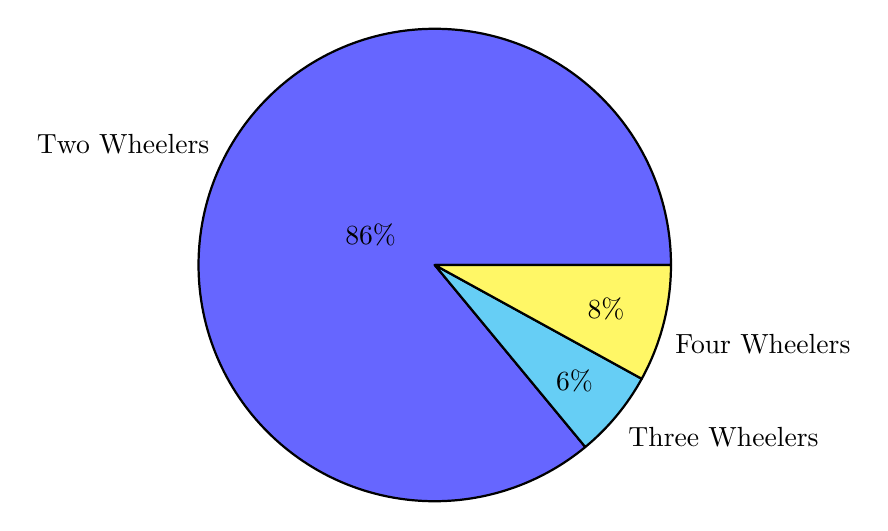
\begin{tikzpicture}
        \pie{86/Two Wheelers, 6/Three Wheelers, 8/Four Wheelers}
    \end{tikzpicture}
    \caption{India EV Automobile distribution}
\end{figure}

\section{Key Players in the Market}
\begin{itemize}

    \item \textbf{Tata Moters:}
    Leading the market with a substantial 72\% share in the electric passenger vehicle segment. Popular models include the Tiago, Nexon, and Tigor.\cite{india_briefing}\cite{jmk_research}
    
    \item \textbf{MG Motor India:}
    Holds about 10.8\% of the market, with notable offerings like the MG ZS and MG Comet. The company is expanding its production capacity and has partnered for charging infrastructure.\cite{india_briefing}\cite{ibef}
    
    \item \textbf{Mahindra \& Mahindra:}
    Accounts for approximately 9\% of the market. The company focuses on electric cars and three-wheelers, with models like the Mahindra XUV400 gaining traction.\cite{india_briefing}\cite{jmk_research}
    
    \item \textbf{Ola Electric:}
    A significant player in the two-wheeler segment, Ola Electric has rapidly captured market share, particularly in registered electric two-wheelers (E2Ws) along with TVS Motor and Ather Energy, which together account for over 65\% of E2W sales.\cite{jmk_research}
    
    \item \textbf{Ather Energy:}
    Known for its high-performance electric scooters, Ather is also investing in charging infrastructure to support its products\cite{imarcgroup}\cite{ibef}
    
    \item \textbf{Hero Electric:}
    This company specializes in electric two-wheelers and has a strong distribution network across India\cite{imarcgroup}
    
    \item \textbf{Hyundai Motor India:}
    This South Korean manufacturer is increasing its footprint in India with plans to launch multiple EV models and establish a robust charging network\cite{india_briefing}\cite{ibef}
    
\end{itemize}

\begin{figure}[h!]
    \centering
    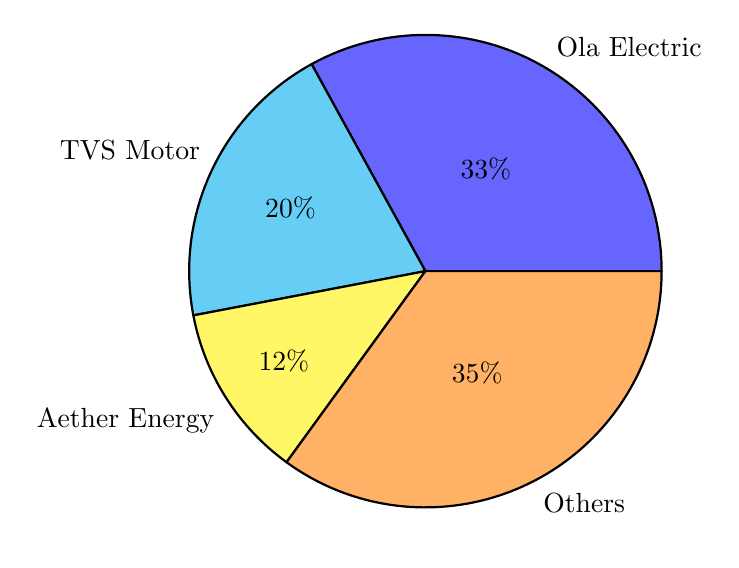
\begin{tikzpicture}
        \pie{33/Ola Electric, 20/TVS Motor, 12/Aether Energy,35/Others}
    \end{tikzpicture}
    \caption{Two Wheeler Distribution}
\end{figure}
\begin{figure}[h!]
    \centering
    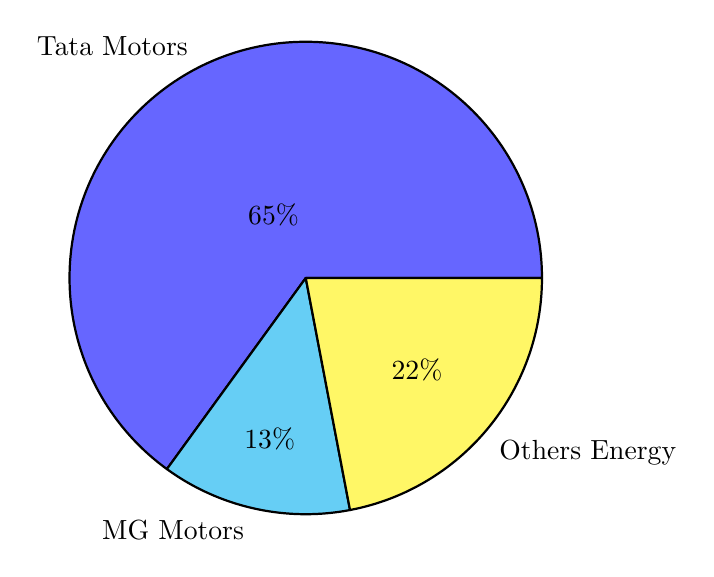
\begin{tikzpicture}
        \pie{65/Tata Motors, 13/MG Motors, 22/Others Energy}
    \end{tikzpicture}
    \caption{Four Wheeler Distribution}
\end{figure}






% Government Policies and Incentives
\chapter{Government Policies and Incentives}
\section{National Electric Mobility Mission Plan (NEMMP)\cite{nemmp}}
The National Electric Mobility Mission Plan (NEMMP) aims to accelerate the adoption of electric vehicles (EVs) in India to achieve environmental sustainability and energy security. Key objectives include:
\begin{itemize}
    \item \textbf{Enhancing Manufacturing:}
    NEMMP promotes local manufacturing of EVs and components, reducing dependency on imports.

    \item \textbf{Promoting Research and Development:}
    It encourages innovation in EV technology, particularly in battery technology and charging infrastructure.

    \item \textbf{Creating Demand:}
    The plan aims to stimulate consumer interest through financial incentives and subsidies.

    \item \textbf{Infrastructure Development:}
    Establishing a robust network of charging stations across urban and rural areas is a priority.
    \\
    Data from the NEMMP indicates that the government envisions achieving a significant percentage of electric vehicles in total vehicle sales by 2030, targeting around 30\% for private cars, 40\% for buses, and 80\% for two-wheelers.
    
\end{itemize}


\section{FAME India Scheme}
The Faster Adoption and Manufacturing of Electric Vehicles in India (FAME) scheme operates in two phases:
\subsection{FAME I}
\begin{itemize}
    \item \textbf{Launch Date:}
    April 2015 with an initial budget of Rs.895 crores. 
    
    \item \textbf{Objectives:}
    To create demand for EVs, support pilot projects, and develop charging infrastructure.

    \item \textbf{Impact:}
   Supported approximately 2.78 lakh EVs, with demand incentives totaling around Rs.343 crores. The scheme also sanctioned 465 electric buses across various cities.
\end{itemize} 

\subsection{FAME II}
\begin{itemize}
    \item \textbf{Launch Date:}
    April 2019 with a budget of Rs.10,000 crores for three years.
    
    \item \textbf{Incentives:}
    \begin{itemize}
        \item Increased subsidy for electric two-wheelers to Rs.15,000 per kWh from Rs.10,000.
        \item Support for 10 lakh e-2Ws, 5 lakh e-3Ws, 55,000 e-4Ws, and 7,000 electric buses.
    \end{itemize}

    \item \textbf{Infrastructure Development:}
    Rs.1,000 crores allocated for establishing charging stations along major highways at intervals of about 25 km.

    \item \textbf{Impact:}
    Supported approximately 2.78 lakh EVs, with demand incentives totaling around Rs.343 crores. The scheme also sanctioned 465 electric buses across various cities.
\end{itemize}

As of July 2023, under FAME II:

\textbf{Total EVs sold:} 832,824
\begin{itemize}
    \item \textbf{Two-wheelers:} 740,722
    \item \textbf{Three-wheelers:} 83,420
    \item \textbf{Four-wheelers:} 8,982
\end{itemize}

\section{State-Level Policies}
Several states have implemented specific policies to support EV growth:
\begin{itemize}
    \item \textbf{Delhi: }
    Offers subsidies up to Rs.30,000 for electric two-wheelers and provides free parking and exemption from road tax. The state aims to have a significant number of electric vehicles on the roads by 2024.
    
    \item \textbf{Maharashtra: }
    Provides incentives for both manufacturers and buyers, including subsidies on purchases and support for charging infrastructure development. The state aims for a target of over 1 lakh EVs by 2025.
    
    \item \textbf{Karnataka: }
    Implements policies promoting electric buses and offers incentives for setting up charging stations. The state has set a goal to have around 1 million EVs by 2030.

\end{itemize}


\section{Tax Incentives and Subsidies}
The Indian government has introduced various tax benefits to encourage EV adoption:
\begin{itemize}
    \item \textbf{Lower GST Rates: }
    Electric vehicles are taxed at a reduced GST rate of 5\%, compared to higher rates for conventional vehicles.

    \item \textbf{Income Tax Benefits: }
    Buyers can claim deductions on interest paid on loans taken to purchase electric vehicles under Section 80EEB of the Income Tax Act.\cite{80eeb}

    \item \textbf{State-Specific Incentives: }
    Many states offer additional subsidies or tax exemptions to further reduce the cost of EVs. For instance, some states provide waivers on road tax and registration fees.
    
\end{itemize}

\section{Charging Infrastructure}
The government is actively working on enhancing the charging infrastructure:
\begin{itemize}
    \item As part of FAME II, over 2,877 charging stations have been sanctioned across various states as of July 2023.
    \item The Ministry of Heavy Industries has also sanctioned Rs.800 crores as capital subsidy to establish public charging stations through Oil Marketing Companies (OMCs), aiming for around 7,432 public charging stations.
    \item Initiatives are underway to develop battery swapping stations as an alternative to traditional charging methods, particularly beneficial for two-wheelers and three-wheelers.
\end{itemize}


These comprehensive policies and initiatives aim to create a conducive environment for the growth of electric vehicles in India while addressing environmental concerns and promoting sustainable transportation solutions.

\begin{figure}[h!]
    \centering
    \begin{tikzpicture}
        \begin{axis}[
            ybar,
            bar width=12pt,
            enlargelimits=0.15,
            ylabel={Percentage BEV penetration},
            xlabel={Categories},
            symbolic x coords={Two-Wheelers, Three-Wheelers, Four-Wheelers},
            xtick=data,
            nodes near coords,
            ymin=0,
            width=12cm,
            height=7cm,
            ymajorgrids=true, % Adds horizontal grid lines
            grid style={dashed, gray!30}, % Style for grid lines
            legend style={
                at={(0.5,-0.15)}, % Position legend below the chart
                anchor=north, 
                legend columns=-1,
                /tikz/column sep=10pt, % Adds horizontal space between entries
                /tikz/row sep=5pt, % Adds vertical space if entries are stacked
            }, % Legend positioning
            group style={group size=2 by 1, horizontal sep=15pt} % Group bars
        ]
        % First data series
        \addplot+[ybar, color=blue, fill=blue!40] coordinates {(Two-Wheelers, 2) (Three-Wheelers, 4) (Four-Wheelers, 1)};
        
        % Second data series
        \addplot+[ybar, color=red, fill=red!40] coordinates {(Two-Wheelers, 20) (Three-Wheelers, 22) (Four-Wheelers, 10)};

         \addplot+[ybar, color=gray, fill=gray!40] coordinates {(Two-Wheelers, 45) (Three-Wheelers, 45) (Four-Wheelers, 20) };
        
        % Add legend
        \legend{2022 , 2026 , 2030 }
        \end{axis}
        
    \end{tikzpicture}
    \caption{Projected BEV Penetration Rates for pessenger vehicles}
\end{figure}








% Market Drivers and Opportunities
\chapter{Market Drivers and Opportunities}
\section{Environmental Concerns and Sustainability}
Increased awareness of climate change and India’s goals to reduce carbon emissions have driven interest in EVs market in India. As Indian government regulates air pollution and environmental degradation, the transition to electric vehicles is heavily prioritized by the government. 

\begin{center}
    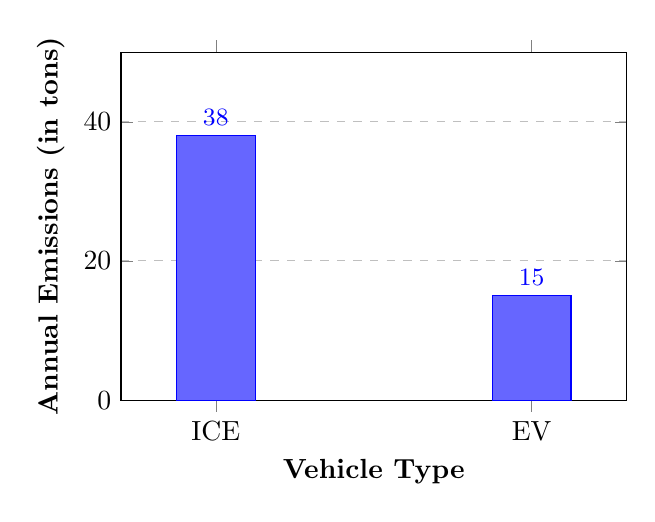
\begin{tikzpicture}
        \begin{axis}[
            ybar,                           % Type of chart (bar chart)
            symbolic x coords={ICE, EV},    % Labels for the x-axis
            xtick=data,                     % Place ticks under each x-label
            ylabel={Annual Emissions (in tons)},                % Label for the y-axis
            xlabel={Vehicle Type},          % Label for the x-axis
            ymin=0,                         % Minimum value for y-axis
            ymax=50,                        % Maximum value for y-axis, slightly above highest value
            bar width=1cm,                  % Width of each bar
            nodes near coords,              % Display values at the top of bars
            every node near coord/.append style={font=\small}, % Font size for labels
            width=8cm,                      % Width of the plot
            height=6cm,                     % Height of the plot
            enlarge x limits=0.3,           % Center bars within the x-axis
            ylabel style={font=\bfseries},  % Bold y-axis label
            xlabel style={font=\bfseries},  % Bold x-axis label
            ymajorgrids=true,               % Adds grid lines to improve readability
            grid style=dashed,              % Dashed style for grid lines
        ]
            % Plot both bars in a single \addplot command to ensure both labels appear
            \addplot+[ybar, fill=blue!60] coordinates {(ICE, 38) (EV, 15)};
        \end{axis}
    \end{tikzpicture}
\end{center}

\begin{itemize}
    \item In regions with a high proportion of renewable energy (like Norway), EVs can have an extremely low carbon footprint.
    \item Conversely, in areas where coal is the primary energy source, such as parts of India or China, the emissions associated with charging can diminish the benefits of EVs. However, even in these scenarios, studies show that EVs still typically outperform ICE vehicles in terms of overall emissions
\end{itemize}

\section{Cost Savings and Efficiency}
Electric Vehicles are very famous for their low operational costs and their cheaper service cost due to the reason that the their are less complexities with a design of an Electric Vehicle as compared to the the design of an internal Combustion Engine (ICE) due to a significantly less amount of moving/mechanical parts. 
\subsection{Lower Operational Costs}
Electric vehicles (EVs) offer significant cost savings over their lifetime compared to traditional internal combustion engine (ICE) vehicles. These savings stem from several key factors:
    \begin{figure}
        \centering
        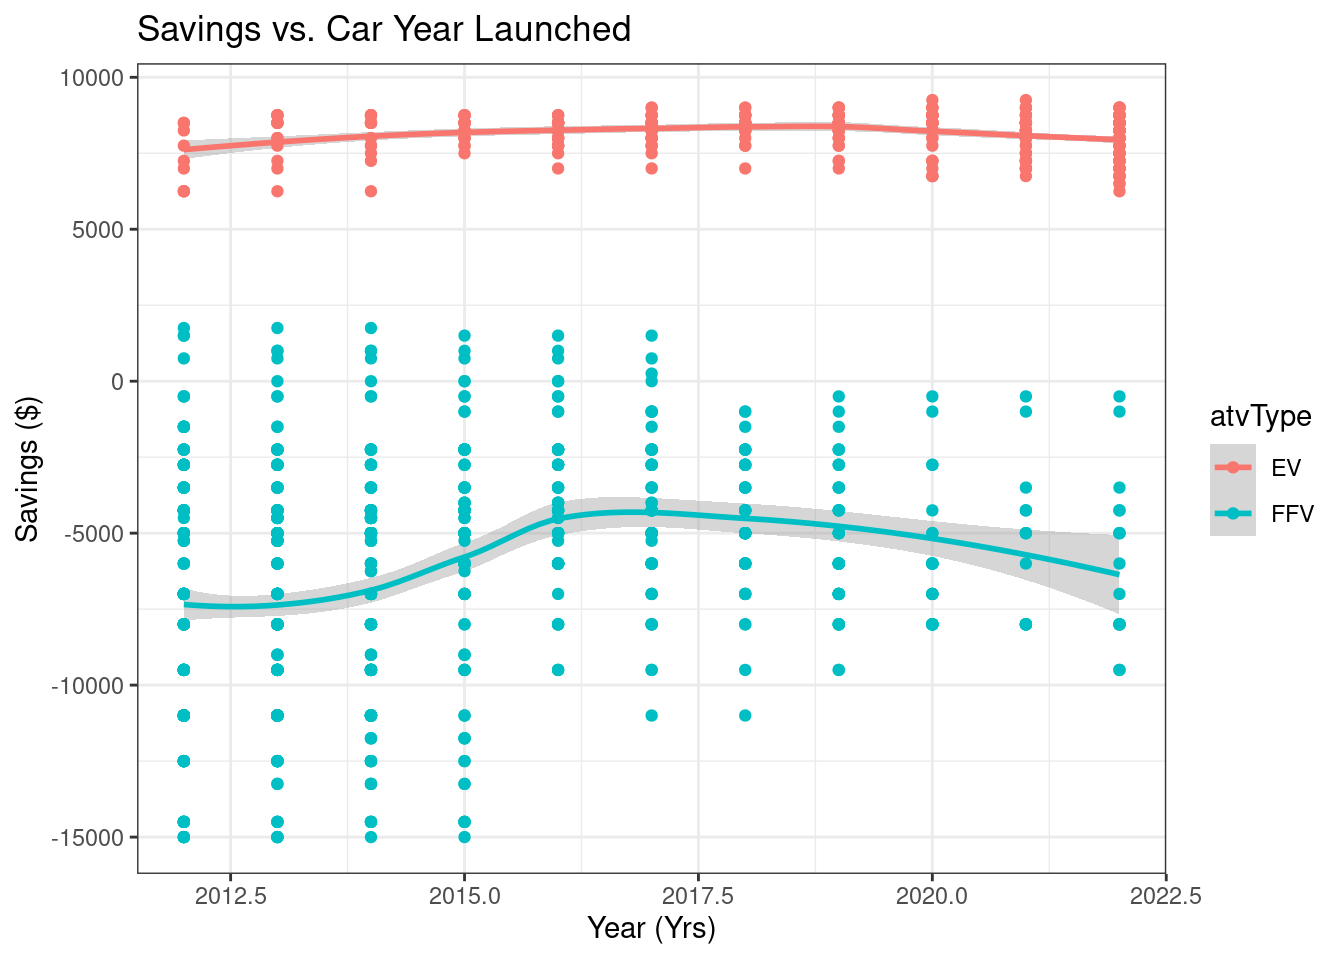
\includegraphics[width=0.8\linewidth]{image.png}
        \caption{Savings vs Car year Launched\cite{rpubs}}
        \label{fig:enter-label}
    \end{figure}


\begin{itemize}
    \item \textbf{Fuel Costs: } The Cost of electricity for charging EVs is very less as compared to the prices of price of Petrol 
    \\ For running a vehicle for 10000km in India, the cost incurred with EVs will be Rs.4,634 per year assuming Rs.7 per unit, while with petrol the amount for this travel will be around Rs.59,000 per year.
    \item \textbf{Maintenance Costs:}
    Evs have lower moving parts, which further leads to less mechanical wear and tear. This causes less downtime with the vehicle and further less maintenance costs. 
    Studies show that EV Owners can save upto Rs.20,000 annually on vehicle maintenance and servicing.
    \item \textbf{Incentives and Tax Credits:}
    Many governments offer financial incentives for purchasing EVs, such as tax credits, rebates, and grants. In the U.S., federal tax credits can be as high as 7,500 USD, while various states offer additional incentives.
\end{itemize}

\subsection{High Efficiency }
Electric vehicles are inherently more efficient than traditional vehicles due to their design and technology:
\begin{itemize}
    \item \textbf{Energy Conversion Efficiency: }
    EVs convert about 60\% to 77\% of the electrical energy from the grid to power at the wheels, compared to ICE vehicles, which convert only about 12\% to 30\% of the energy stored in gasoline into movement.
    \\ This higher efficiency means that EVs can travel further distance with the same amount of energy.
    \item \textbf{Regenerative Braking: }EVs utilize regenerative braking systems that capture energy usually lost during braking and convert it back into usable electricity for the battery. This feature enhances overall efficiency and extends driving range.
    \item \textbf{Performance Benefits: }Electric motors provide instant torque, allowing for quicker acceleration compared to traditional engines. This performance advantage contributes not only to a better driving experience but also to efficient energy use.
    \end{itemize}

\section{Technological Advancements}
Recent advancements in the field of Batteries, Motors and Charging technology has led to a significant enhancement in the practicality and accessibility of Electric vehicles. 
\subsection{Advances in Battery Technology}
There have been a lot of rapid growth in the field of battery technology including development of new battery compounds and ways to integrate batteries in vehicles. 
\begin{itemize}
    \item \textbf{Increased Energy Density: }
    Modern lithium-ion batteries now offer energy densities exceeding 250 Wh/kg, allowing EVs to achieve longer ranges. For example, the Tesla Model 3 can travel over 350 miles on a single charge, addressing range anxiety—a major barrier to EV adoption.

    \item \textbf{Faster Charging Capabilities: }
    Innovations in fast-charging technology enable EVs to recharge more quickly. DC fast chargers can deliver power outputs between 90 kW and 400 kW, allowing some vehicles to charge from 20\% to 80\% in just 15 to 30 minutes. This rapid charging capability makes it feasible for drivers to integrate charging into their daily routines, such as during lunch breaks or grocery shopping

    \item \textbf{Battery Longevity: }
    Advances in battery management systems and materials have improved the lifespan of EV batteries. Many modern batteries are designed to last over 480000 km, significantly reducing the total cost of ownership for EVs.

    \item \textbf{Solid-State Batteries: }
    Research into solid-state batteries promises even greater improvements, with potential energy densities of up to 500 Wh/kg and faster charging times, while also enhancing safety by reducing flammability risks associated with liquid electrolytes
    
\end{itemize}


\subsection{Fast Charging Solution}
The development of fast charging infrastructure is crucial for making EVs more practical for everyday use, some of the developements in this field include,
\begin{itemize}
    \item \textbf{DC Fast Charging Stations: }
    The proliferation of DC fast charging stations is critical for reducing charging times. For instance, stations can charge an EV to 80\% capacity in approximately 30 minutes, making long-distance travel more feasible

    \item \textbf{Mobile Charging Stations: }
    Companies are introducing mobile DC fast chargers that can be deployed quickly and easily at various locations, including service stations and events. These portable solutions can charge an average EV in about 30 minutes, improving access to charging facilities where infrastructure may be lacking.

    \item \textbf{Smart Charging Networks: }
    Advanced charging networks are being developed that allow users to track and manage their charging sessions via mobile apps, optimizing energy use and providing real-time information on charger availability. This technology facilitates better integration with renewable energy sources, reducing overall emissions associated with charging

    \item \textbf{Standardization of Charging Connectors: }
    The adoption of standardized connectors like CCS (Combined Charging System) facilitates compatibility across different vehicle models and charging stations, further enhancing the user experience and accessibility of EV charging infrastructure. 
\end{itemize}



\section{Growing Consumer Demand}
The Indian market is witnessing a significant shift in the consumer preferences towards greener and more cost-effective transportation solutions.
\subsection{Shift towards Electric Vehicle (EVs)}
\begin{itemize}
    \item The demand for electric vehicles in India is rapidly increasing, with projections indicating that the country aims for 30\% electrification of all vehicles by 2030. This target is supported by government initiatives such as the FAME India scheme, which provides incentives for EV adoption.
    \item In 2023, the Indian EV market was valued at approximately 8 billion USD, with expectations to grow to 23.38 billion USD by 2024 and 117.78 billion USD by 2032. This growth is driven by rising consumer awareness of the environmental benefits of EVs and favorable government policies promoting electric mobility .
\end{itemize}

\subsection{Cost-Effectiveness:}
\begin{itemize}
    \item Consumers are increasingly recognizing the long-term cost savings associated with EV ownership. Operating costs for EVs are significantly lower than those for traditional internal combustion engine vehicles. For example, the cost of electricity for charging an EV is approximately Rs.2.52 per mile, compared to about Rs.11.7 per mile for petrol vehicles. 
    \item The operational cost benefits of electric commercial vehicles, such as buses and trucks, are also encouraging fleet operators to transition to electric options, further enhancing their appeal in urban transportation and logistics sectors.
\end{itemize}

\subsection{Health and Environmental Awareness:}
\begin{itemize}
    \item With urban air quality deteriorating due to pollution from conventional vehicles, consumers are increasingly motivated to opt for cleaner alternatives. The Indian government’s commitment to reducing carbon emissions aims to cut down on harmful pollutants like nitrogen oxides (NOx) and particulate matter (PM), which contribute to serious health issues.
    \item A report predicts that improved logistics practices, including the adoption of electric vehicles, could save India up to 10 gigatons of CO2 emissions by 2050 while significantly reducing PM and NOx emissions.
\end{itemize}

\section{Job Creation Potential}
The growing electric vehicle (EV) sector in India is poised to create substantial job opportunities across various domains, including manufacturing, services, and infrastructure.

\subsection{Projected Job Growth: }
\begin{itemize}
    \item \textbf{Direct and Indirect Job Creation: }
    \begin{itemize}
        \item By 2030, the EV industry is projected to generate 10 million direct jobs and an additional 50 million indirect jobs. This indicates a total potential of 60 million jobs linked to the burgeoning EV ecosystem .\cite{PeopleLogic}\cite{DownToEarth}
        \item The Society of Indian Automobile Manufacturers (SIAM) estimates that around 200,000 skilled workers will be needed by 2030 to support the government's vision of achieving 30\% EV penetration in the automotive sector.\cite{EconomicTimes}
    \end{itemize}
    \item \textbf{Sector-Specific Opportunities: }
    \begin{itemize}
        \item The manufacturing sector will see significant job growth as companies transition from traditional internal combustion engine (ICE) vehicles to EVs. This includes roles in assembling electric motors, battery packs, and integrating electronic components.
        \item Research and development (R\&D) positions are expected to surge, particularly for engineers and scientists focused on advanced battery technologies and electric drivetrain.
    \end{itemize}
    \item \textbf{Emerging Roles: }
    \item New job roles are anticipated in areas such as charging infrastructure installation, maintenance, and operations. As the government and private entities invest in expanding charging networks, there will be a demand for electrical engineers and technicians \cite{PeopleLogic}
    \item Sales and marketing roles will evolve as consumer buying behaviors change. Professionals who understand both technology and consumer needs will be crucial for educating potential buyers about EVs.
\end{itemize}

\newpage
\subsection{Skill Development Needs}
\begin{itemize}
    \item \textbf{Skill Gaps: }
    \begin{itemize}
        \item A report indicates that 43\% of the technical competencies required for EVs differ significantly from those needed for ICE vehicles, necessitating fresh skill development initiatives.\cite{EconomicTimes}
        \item The demand for skilled professionals is expected to rise sharply, with estimates suggesting that India needs to add 30,000 EV-ready workers annually until 2030 to meet localization goals for EV components.\cite{EconomicTimes}
    \end{itemize}
    \item \textbf{Training Investments: }
    The total investment required for hiring and training the workforce in the EV sector is projected to be around Rs.13,552 crore, with significant portions allocated for both hiring costs and training programs \cite{EconomicTimes}
\end{itemize}



% Challenges Facing the EV Market
\chapter{Challenges Facing the EV Market}
\section{Charging Infrastructure}
The limited availability of charging stations in both urban and rural areas remains a major barrier to electric vehicle (EV) adoption in India. Despite the government's push for electric mobility, the current charging infrastructure is insufficient to meet the needs of potential EV buyers.

\begin{itemize}
    \item \textbf{Current State of Charging Infrastructure: }
    As of 2023, India has approximately 8,738 operational charging stations, but these are predominantly located in urban centers. This uneven distribution creates accessibility issues for users in rural and semi-urban areas, leading to concerns about finding charging points when needed.\cite{evPedia}\cite{emobility+}
    \item \textbf{Rural Accessibility: }
    In rural areas, the lack of access to reliable electricity grids further complicates the installation of charging stations. Many remote locations lack the necessary infrastructure to support charging facilities, making it difficult for EV owners in these regions to recharge their vehicles \cite{evPedia}
\end{itemize}

\section{High Initial Costs}
The higher upfront costs of EVs compared to traditional vehicles continue to be a significant barrier to adoption in India:
\begin{itemize}
    \item \textbf{Price Sensitivity: }
    Indian consumers are generally price-sensitive, and the initial cost of electric vehicles often exceeds that of internal combustion engine (ICE) vehicles. This price disparity can deter potential buyers from making the switch to electric mobility.\cite{emobility+} \cite{decan}
    \item \textbf{Government Subsidies: }
    To address this issue, various state governments have introduced subsidies and incentives for EV buyers. For instance, Delhi provides a subsidy of up to Rs.1.5 lakhs for electric vehicle purchases, making them more accessible. However, these incentives may not be sufficient to overcome the overall cost barrier for many consumers.\cite{emobility+}
\end{itemize}

\section{Range Anxiety}
Concerns over the driving range of EVs and the need for widespread fast-charging networks further complicate consumer acceptance:
\begin{itemize}
    \item \textbf{Driving Range Limitations: }
    While many modern EVs offer ranges exceeding 300 kilometers, potential buyers still express concerns about whether they can complete longer trips without encountering charging issues. \cite{emobility+}\cite{codibly}
    \item \textbf{Need for Fast Charging Networks: }
    The establishment of a robust fast-charging network is essential for alleviating range anxiety. Currently, most charging stations are slow chargers that require significant time to recharge vehicles, which can be inconvenient for users on tight schedules.\cite{evPedia} \cite{codibly}
\end{itemize}

\section{Battery Technology and Disposal}
Environmental concerns related to the disposal and recycling of lithium-ion batteries present additional challenges:
\begin{itemize}
    \item \textbf{Battery Lifespan and Recycling: }
    As EV adoption increases, so does the need for effective recycling solutions for lithium-ion batteries once they reach the end of their life cycle. Current recycling processes are not fully developed in India, raising concerns about environmental impacts if batteries are improperly disposed of. \cite{emobility+}\cite{decan}
    \item \textbf{Resource Extraction Concerns: }
    The extraction of materials used in battery production, such as lithium and cobalt, raises ethical and environmental concerns that need addressing as demand for EVs grows.s\cite{codibly}
\end{itemize}

% Competitive Landscape
\chapter{Competitive Landscape}
\section{Local vs Global Players}
The Indian electric vehicle (EV) market is characterized by a mix of domestic manufacturers and global competitors, each vying for a share of the rapidly expanding market.
\subsection{Domestic Manufacturers: }
\begin{itemize}
    \item \textbf{Tata Motors: }
    A leader in the Indian EV space, Tata Motors has launched several successful models, including the Nexon EV and Tigor EV. The company is actively expanding its EV portfolio and aims to increase production capacity significantly
    \item \textbf{Mahindra Electric: }
    Known for its focus on electric mobility, Mahindra has introduced models like the eVerito and eKUV100, targeting both personal and commercial segments. The company is also investing in battery technology to enhance its offerings.
    \item \textbf{Ather Energy: }
    A startup focusing on electric scooters, Ather has gained attention for its innovative designs and technology-driven approach. Its Ather 450X model is popular among urban consumers for its performance and smart features.
\end{itemize}
\subsection{Global Manufacturers: }
\begin{itemize}
    \item \textbf{Tesla: }
    The American EV giant is exploring entry into the Indian market, which could significantly disrupt local dynamics. Tesla’s reputation for high-performance electric vehicles positions it as a formidable competitor.
    \item \textbf{Volkswagen Group: }
    With plans to introduce a range of electric models in India, Volkswagen aims to leverage its global expertise in EV technology to capture market share.
    \item \textbf{Hyundai: }
    Already active in the Indian market with the Kona Electric, Hyundai plans to expand its electric offerings, capitalizing on its established brand presence.
\end{itemize}

\section{Innovation and Differentiation}
Key product and technological innovations in the EV market in India.
\begin{itemize}
    \item \textbf{Battery Technology: }
    \begin{itemize}
        \item Advances in battery technology are central to enhancing vehicle performance and reducing costs. Domestic manufacturers are increasingly focusing on developing indigenous battery solutions to lower dependency on imports and improve supply chain resilience
        \item Companies like Tata Power are investing in battery recycling technologies to address environmental concerns associated with lithium-ion batteries.
    \end{itemize}
    \item \textbf{Smart Features: }
    Many EV manufacturers are integrating smart technologies into their vehicles, such as connected car features, advanced driver-assistance systems (ADAS), and over-the-air software updates. This not only enhances user experience but also improves vehicle performance and safety.
    \item \textbf{Sustainability Initiatives: }
    Manufacturers are adopting sustainable practices in production processes, including using recyclable materials and implementing energy-efficient manufacturing techniques. This commitment to sustainability resonates with environmentally conscious consumers.
\end{itemize}

\section{EV Ecosystem}
The broader ecosystem supporting electric vehicles in India encompasses various components that facilitate growth and adoption:
\begin{itemize}
    \item \textbf{Battery Suppliers: }
    A robust network of battery suppliers is essential for the EV industry. Companies like Ather Energy are focusing on developing high-performance batteries tailored for Indian conditions, ensuring reliability and efficiency.
    \item \textbf{Charging Infrastructure: }
    \begin{itemize}
        \item The expansion of charging infrastructure is critical for supporting EV adoption. The government’s Faster Adoption and Manufacturing of Hybrid and Electric Vehicles (FAME) scheme aims to incentivize the establishment of charging stations across urban and rural areas.
        \item Private players like Tata Power and ChargePoint are actively investing in charging networks, aiming to increase accessibility and convenience for users.
    \end{itemize}
    \item \textbf{Software Providers: }
    The integration of software solutions is crucial for managing charging networks, vehicle diagnostics, and customer engagement. Companies specializing in software development for connected vehicles are becoming increasingly important in the EV ecosystem.
    \item \textbf{Public-Private Partnerships (PPP): }
    Collaboration between government entities and private companies is essential for building a comprehensive EV ecosystem. Initiatives that promote investment in charging infrastructure and battery manufacturing can accelerate the transition to electric mobility.

\end{itemize}

% Future Outlook
\chapter{Future Outlook}
\section{Growth Projections}
India's electric vehicle (EV) market is anticipated to experience significant growth over the next 5-10 years. By 2030, the government aims for 40\% of new buses to be electric, which translates to approximately 800,000 electric buses replacing diesel models. As of early 2024, India had registered around 8,583 electric buses, with projections indicating a dramatic increase in adoption as government incentives and infrastructure improve. The overall EV market share is expected to rise from its current low levels, particularly in urban areas where electric buses are being prioritized.\cite{changingTransport}


\section{Emerging Trends}
There are many trends which are visible in the current scenario :
\begin{itemize}
    \item \textbf{Electric Two-Wheelers: }
    The two-wheeler segment is seeing rapid growth, driven by increasing urbanization and the need for sustainable transportation options. Government subsidies and rising fuel costs are encouraging consumers to switch to electric models
    \item \textbf{Electric Buses: } The introduction of electric buses in major cities is gaining momentum. Initiatives like the PM e-Bus Sewa aim to deploy thousands of electric buses across urban centers\cite{changingTransport}
    
\end{itemize}


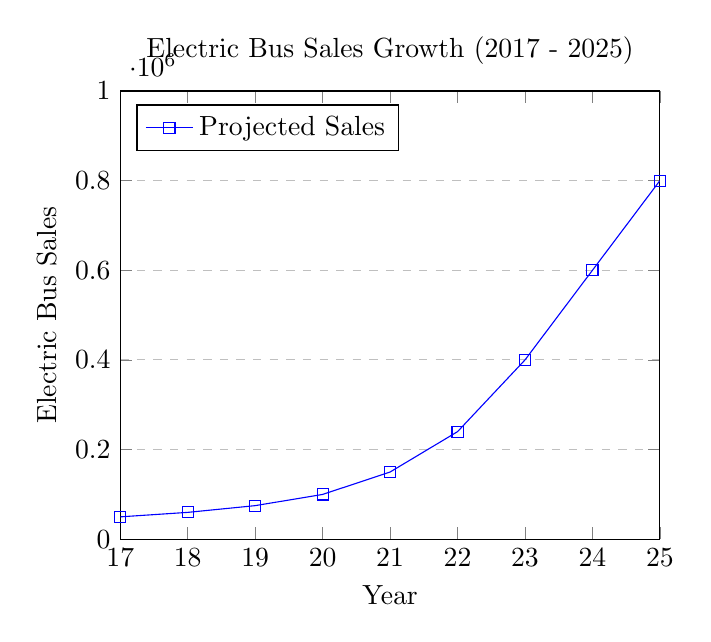
\begin{tikzpicture}
\begin{axis}[
    title={Electric Bus Sales Growth (2017 - 2025)},
    xlabel={Year},
    ylabel={Electric Bus Sales},
    xmin=17, xmax=25,
    ymin=0, ymax=1000000,
    xtick={17,18,19,20,21,22,23,24,25},
    ytick={0,200000,400000,600000,800000,1000000},
    legend pos=north west,
    ymajorgrids=true,
    grid style=dashed,
]
\addplot[
    color=blue,
    mark=square,
    ]
    coordinates {
    (17,50000)(18,60000)(19,75000)(20,100000)(21,150000)(22,240000)(23,400000)(24,600000)(25,800000)
    };
\legend{Projected Sales}
\end{axis}
\end{tikzpicture}






\section{Impact of Autonomous and Connected Vehicles}
The potential for autonomous and connected vehicle technologies in India is significant, with various factors contributing to their expected impact on transportation systems and urban mobility
\subsection{Enhancement in Public Transport and Traffic Management}
\begin{itemize}
    \item \textbf{Efficiency Improvements: }
    Autonomous electric vehicles (EVs) can streamline public transport operations by optimizing routes and schedules based on real-time data. This can lead to reduced wait times and improved service reliability, making public transport more attractive to users.
    \item \textbf{Traffic Management: }
    Connected vehicles equipped with Vehicle-to-Everything (V2X) technology can communicate with traffic signals, other vehicles, and infrastructure to enhance traffic flow and reduce congestion. This capability is crucial in densely populated urban areas where traffic jams are common.
    \item \textbf{Cost Reduction for Fleet Operators: }
    The adoption of autonomous EVs can significantly lower operational costs for fleet operators by minimizing labor costs and reducing fuel expenses through efficient energy use.
\end{itemize}

\subsection{Safety and User-Experience }
\begin{itemize}
    \item \textbf{Increased Safety: }
    Advanced Driver Assistance Systems (ADAS) integrated into connected vehicles can help prevent accidents by providing features such as collision avoidance, lane departure warnings, and automatic emergency braking. The adoption of these technologies is expected to grow, with a reported 70\% year-on-year increase in vehicles featuring Level 2 autonomy as of 2023.
    \item \textbf{Enhanced User Experience: }
    Connected vehicles offer features that improve the overall driving experience, such as personalized settings, predictive maintenance alerts, and infotainment options. As consumer demand for connectivity rises, automakers are increasingly integrating these technologies into their offerings.
\end{itemize}

\subsection{Challenges with Autonomous Driving}
\begin{itemize}
    \item \textbf{Poor Road Conditions: }
    Indian roads often suffer from potholes, uneven surfaces, and inadequate maintenance, making it difficult for autonomous vehicles to navigate safely and effectively. The lack of well-maintained infrastructure poses a challenge for the sensors and algorithms that guide these vehicles.
    \item \textbf{Insufficient Charging Infrastructure: }
    For electric autonomous vehicles, the charging infrastructure is lagging significantly. While there have been advancements for smaller electric vehicles, dedicated charging facilities for buses and larger vehicles are still underdeveloped
    \item \textbf{Heterogeneous Traffic: }
    Indian roads are shared by a diverse range of vehicles, including bicycles, rickshaws, and heavy trucks, which complicates the development of reliable autonomous navigation systems. The chaotic nature of traffic patterns can lead to unpredictable situations that autonomous systems must be able to handle.
    \item \textbf{Non-compliance with Traffic Regulations: }
    There is a prevalent disregard for traffic rules among many drivers in India, such as jaywalking and ignoring signals. This behavior creates an unpredictable environment that is challenging for autonomous vehicles to navigate safely.
    \item \textbf{Lack of Legal Framework: }
    Current laws, such as the Motor Vehicles Act of 1988, do not accommodate autonomous vehicles. There is no provision for testing or operating these vehicles legally on Indian roads, which hampers innovation and development efforts.
    \item \textbf{Liability Issues: }
    Determining liability in the event of an accident involving an autonomous vehicle presents complex legal challenges. Questions arise regarding whether the vehicle owner, manufacturer, or software developer should be held responsible.
\end{itemize}
There are other challenges such as Public Skepticism, Price sensitivity, need for Technological Advancements and talent acquisition which are affecting the current growth of Autonomous driving in India. 


\section{International Collaborations}
India's push towards electrification in the automotive sector is significantly bolstered by international collaborations. These partnerships are crucial for accelerating technology transfer, enhancing local manufacturing capabilities, and developing robust infrastructure. Here’s a detailed exploration of the current landscape of international collaborations in India's EV sector.
\begin{itemize}
    \item \textbf{Ahamani EV Technology: }
    This company is actively engaging with Indian automotive giants to facilitate technology transfer. Their initiatives include establishing a megawatt-scale battery plant, which will support both electric vehicles and drones, thereby enhancing local manufacturing capabilities and innovation in the EV sector.
    \item \textbf{ISRO Collaborations: }
    The Indian Space Research Organisation (ISRO) has been instrumental in transferring lithium-ion battery manufacturing technology to various Indian companies. This initiative aims to bolster domestic production capabilities and reduce reliance on imports.
    \item \textbf{Tata Motors and Mahindra \& Mahindra Initiatives: }
    Major Indian automakers like Tata Motors and Mahindra \& Mahindra are actively developing autonomous vehicle technologies. Tata Motors is working on a framework for semi-autonomous vehicles while also collaborating with Cognizant Technologies to create indigenous prototypes.
    \item \textbf{Swaayatt Robots: }
    Founded by IIT Roorkee graduate Sanjeev Sharma, Swaayatt Robots is developing advanced algorithms for autonomous driving. Their approach is focused on achieving Level 5 autonomy, where no human intervention is needed.
\end{itemize}

% Recommendations
\chapter{Recommendations}
\section{For Manufacturers}
To reduce costs and improve battery efficiency, EV manufacturers in India can adopt several strategies:
\begin{itemize}
    \item \textbf{Invest in Local Battery Manufacturing: }
    Establishing domestic battery manufacturing facilities can significantly reduce costs associated with imports. Research indicates that local production can lower battery costs by approximately 20-30\% due to reduced logistics and tariffs.\cite{icrier}
    \item \textbf{Enhance Battery Efficiency: }
    Manufacturers should focus on improving the energy density of batteries. For instance, increasing the efficiency of EVs to achieve up to 4.2 miles per kWh (as seen with models like the Hyundai Ioniq 6) can reduce battery size and costs by nearly 40\%, translating to savings of about USD 4,800 per vehicle.
    \item \textbf{Focus on Recycling and Circular Economy: }
    Developing robust recycling processes for used batteries can lower demand for new materials and reduce costs. Currently, less than 1\% of lithium batteries are recycled; improving this could significantly impact material sourcing and overall expenses.
\end{itemize}


\section{For Policymakers}
Policymakers play a crucial role in fostering an environment conducive to EV growth through strategic initiatives:
\begin{itemize}
    \item \textbf{Continue Subsidies and Tax Breaks: }
    Extending existing subsidies for EV purchases can incentivize consumers to choose electric over traditional vehicles. For example, maintaining or increasing the current subsidy levels could boost sales by as much as 30\% annually.
    \item \textbf{Enhance Charging Infrastructure Development: }
    Investing in charging infrastructure is critical for supporting the growing EV market. The government should aim to establish at least 1 million public charging stations by 2030 to ensure accessibility and convenience for users.
    \item \textbf{Standardization of Battery Technologies: }
    Implementing standardized battery specifications can facilitate interoperability among different EV models, particularly in public transportation systems like buses, enhancing user confidence and adoption rates.
    \item \textbf{Research Grants for Efficiency Improvements: }
    Allocating funds for research into battery technology improvements can lead to breakthroughs that reduce costs and enhance performance. This could include grants focused on developing next-generation lithium-sulfur or solid-state batteries.
\end{itemize}


\section{For Investors}
Investors have numerous opportunities to capitalize on the growth of the Indian EV market:
\begin{itemize}
    \item \textbf{Invest in Startups Focused on EV Technology: }
    The Indian startup ecosystem is burgeoning with innovative companies focused on electric mobility solutions, including battery technology, charging infrastructure, and software development for autonomous vehicles. Investing in these startups can yield significant returns as demand grows.
    \item \textbf{Funding Charging Infrastructure Projects: }
    With the government aiming for extensive charging networks, investing in companies that develop or operate charging stations presents a lucrative opportunity. The market for charging infrastructure is expected to grow at a CAGR of over 30\%, reaching approximately USD 10 billion by 2025.
    \item \textbf{Engage in Joint Ventures with Established Automakers: }
    Collaborating with established automotive manufacturers looking to expand their electric offerings can provide investors with access to resources, technology, and market expertise.
\end{itemize}


% Conclusion
\chapter{Conclusion}
The Electric Vehicle (EV) market in India is poised for substantial growth, driven by increasing environmental awareness, government support, and advancements in technology. This report highlights key factors influencing the market, including:
\begin{itemize}
    \item \textbf{Government Initiatives: }
    The Indian government's commitment to promoting EVs through various subsidy schemes, policies like the National Electric Mobility Mission Plan (NEMMP), and the Faster Adoption and Manufacturing of Electric Vehicles (FAME) initiative has significantly contributed to market growth.
    \item \textbf{Market Segmentation: }
    The analysis of different segments—passenger vehicles, two-wheelers, three-wheelers, and commercial vehicles—reveals varying levels of consumer adoption and market dynamics. The dominance of two-wheelers and the emerging interest in electric cars signify a shift in consumer preferences.
    \item \textbf{Key Players: }
    Major companies such as Tata Motors, MG Motor, Mahindra \& Mahindra, Ola Electric, and others are leading the market with innovative products and expanding production capacities, enhancing competition and consumer choices.
    \item \textbf{Challenges and Opportunities: }
    While challenges such as charging infrastructure, battery costs, and consumer awareness persist, there are significant opportunities for stakeholders to innovate and create solutions that can accelerate EV adoption.

\end{itemize}

In conclusion, the EV market in India presents a promising landscape for investment and development. Continued collaboration between government, industry players, and consumers is essential to overcome challenges and harness the full potential of electric mobility in the country.

\newpage


% Appendices
\appendix
\chapter{Appendices}
\section{Data Tables}
\begin{longtable}{|l|l|l|}
\hline
\textbf{Year} & \textbf{Total EV Sales (Units)} & \textbf{Market Growth (\%)} \\
\hline
2018 & 56,000 & - \\
2019 & 75,000 & 33.93 \\
2020 & 130,000 & 73.33 \\
2021 & 170,000 & 30.77 \\
2022 & 220,000 & 29.41 \\
2023 & 350,000 & 59.09 \\
\hline
\end{longtable}
\section{Glossary}
\begin{itemize}
    \item \textbf{Electric Vehicle (EV):} A vehicle that operates on electric power, typically using an electric motor instead of a conventional internal combustion engine, resulting in reduced emissions and lower operational costs.
    
    \item \textbf{FAME (Faster Adoption and Manufacturing of Electric Vehicles):} A government initiative in India aimed at promoting electric vehicle adoption through incentives and subsidies to consumers and manufacturers.
    
    \item \textbf{FAME-I:} The first phase of the FAME initiative, launched in 2015, which focused on incentivizing the purchase of electric and hybrid vehicles.
    
    \item \textbf{FAME-II:} The second phase of the FAME initiative, introduced in 2019, which expands the scope of incentives and includes support for charging infrastructure development.
    
    \item \textbf{National Electric Mobility Mission Plan (NEMMP):} A government policy aimed at creating a comprehensive framework for promoting electric mobility in India, including manufacturing and adoption strategies.
    
    \item \textbf{Production Linked Incentive (PLI):} A government scheme designed to encourage domestic manufacturing and attract investment in electric vehicle production and battery manufacturing.
    
    \item \textbf{Range Anxiety:} The fear or concern of electric vehicle users regarding the vehicle's ability to travel a sufficient distance on a single charge, often leading to hesitance in adopting EVs.
    
    \item \textbf{Battery Electric Vehicle (BEV):} A type of electric vehicle that is fully powered by an electric battery, with no internal combustion engine, and must be charged from an external power source.
    
    \item \textbf{Plug-in Hybrid Electric Vehicle (PHEV):} A hybrid vehicle that can be charged from an external power source and can operate on electric power alone for a limited range, in addition to conventional fuel.
    
    \item \textbf{Charging Infrastructure:} The network of charging stations and facilities that enable electric vehicle users to charge their vehicles.
    
    \item \textbf{Market Growth Rate:} The percentage increase in sales or adoption of electric vehicles over a specific time period, indicating market trends and consumer acceptance.
    
    \item \textbf{Consumer Survey:} A research tool used to gather opinions, behaviors, and preferences of consumers regarding electric vehicles, helping to inform market strategies.
    
    \item \textbf{EV Market Players:} Companies and organizations involved in the manufacturing, sale, or promotion of electric vehicles, including traditional automotive companies and new startups.
    
    \item \textbf{Sustainability:} The ability to meet present needs without compromising the ability of future generations to meet their own needs, often associated with environmental preservation and responsible resource management.
    
    \item \textbf{Government Incentives:} Financial or non-financial benefits offered by the government to encourage the adoption and manufacturing of electric vehicles, such as tax rebates or grants.
    
    \item \textbf{Two-Wheeler Electric Vehicle:} Electric vehicles designed for two riders, such as electric scooters and motorcycles, which are becoming increasingly popular in urban areas.
\end{itemize}


\section{References}
References are listed in the last page under Bibliography section. This Report utilized multiple reports, website articles, open researches and data analyses projects.
\printbibliography

\end{document}
